Según Kirk \cite{Kir12}, la visualización de datos es un proceso de diseño mediante el cual se codifican y presentan los datos de tal forma que se aprovechan las capacidades de percepción visuales para maximizar la efectividad y eficiencia con la que nuestro cerebro procesa información y produce conocimiento.

Según Ilinnsky y Steele \cite{Ste11}, la visualización es un medio útil para examinar, entender y transmitir la información por diversas razones, entre las cuales están:

\begin{itemize}
  \item Aprovechar las capacidades de los sistemas visuales para transmitir una gran cantidad de información al cerebro rápidamente.
  \item Hacer uso de las capacidades del cerebro para identificar patrones y comunicar relaciones y significados.
  \item Inspirar mayores exploraciones y nuevas preguntas.
  \item Ayudar a identificar sub-problemas.
  \item Identificar tendencias y valores extremos, descubrir o buscar puntos de interés en un mar de datos, etc. 
\end{itemize}

Una función clave de la visualización de datos es mover información del punto A al punto B. En la visualización exploratoria de datos el punto A son los datos y el punto B es la mente del diseñador. En la visualización explicativa el punto A es la mente del diseñador y el punto B es la mente del usuario.

\section{Clasificación}
Las visualizaciones de datos pueden clasificarse de diversas maneras. Kirk \cite{Kir12} establece clasificaciones según la intención de la visualización; función y tono. Por su parte, Ilinnsky y Steele \cite{Ste11} proponen una clasificación según la complejidad de la visualización.

\subsection{Según su función}

Involucra la experiencia funcional que se puede crear entre el diseño, los datos y el usuario. Se disponen de las siguientes tres alternativas:

\begin{itemize}
  \item Cuando la función es explicar.
  \item Cuando la función es explorar.
  \item Cuando la expresión es la expresión visual.
\end{itemize}

\subsubsection{Cuando la función es explicar}

En este caso se trata de comunicar información al usuario mediante una narrativa enfocada y específica. Las visualizaciones de este tipo se conocen como visualizaciones explicativas.

\subsubsection{Cuando la función es explorar}

Las visualizaciones de este tipo, denominadas visualizaciones de exploración, ofrecen al usuario un ambiente de exploración visual de datos que le permite sacar sus propios patrones, relaciones, tendencias y conocimientos.

Una funcionalidad que permite generar una experiencia verdadera de exploración es la interactividad. Con ella el usuario es capaz de sumergirse en un reto dinámico de solución de problemas. Algunas de estas de funcionalidades son el filtrado, ordenamiento, selección (brushing), ajuste de variables y modificación de vista.

\subsubsection{Cuando la función es la expresión visual}

En este caso se hace uso de los datos como materia prima para la expresión artística. Esto difiere de los casos anteriores cuya finalidad es esencialmente informar.

\subsection{Según su tono}

Esta clasificación se enfoca en la respuesta emocional y en el tipo de estímulo que se está intentando crear. Existen dos tonos diferenciados.

Pragmático y analítico: son aquellas visualizaciones que se enfocan en la necesidad de un diseño que entregue una representación de datos de forma rápida, eficiente y precisa. En este caso, el objetivo principal es informar.
Emotiva y abstracta: son aquellas enfocadas en la experiencia estética que ilustra la historia general de los datos. En muchos casos sacrifican el nivel de detalle con el fin de generar un impacto emocional o hacer énfasis en un hecho. Sin embargo, preservan la visión general.

\subsection{Según su complejidad}

Esta clasificación categoriza las visualizaciones según el número de variables que representan. Por ejemplo, un gráfico de precio de acción (stock) contiene cuatro propiedades: fecha, precio, compañía y capitalización de mercado. Cada una es una dimensión distinta de los datos, que puede ser codificada por separado, usando una propiedad visual diferente.

\section{Proceso de Diseño}

Kirk \cite{Kir12} propone un proceso de diseño para la visualización de datos que incluye las siguientes fases: concepción del proyecto, análisis de los datos y diseño. El método pretende ser independiente de la tecnología y hace énfasis en la conceptualización, razonamiento y la toma de decisiones. Evita cualquier sentido de instrucción dogmática y se enfoca en ofrecer un conjunto de pautas generales. Se pretende que el método sea adoptado con flexibilidad, basado en el propio juicio y discreción.

\subsection{FASE I: Concepción del proyecto}

Antes de acometer cualquier proceso de diseño, se debe estar claro sobre la motivación que da origen al proyecto. Esto involucra identificar la audiencia y sus necesidades. Es también fundamental revisar cuidadosamente la intención del proyecto y cómo se define la función y tono de la visualización.

\subsection{FASE II: Análisis}

Esta fase consta de dos actividades. En la primera se adquieren, preparan y estudian los datos. En la segunda se lleva a cabo un análisis visual con el fin de descubrir las historias claves contenidas en los datos.

\subsubsection{Preparando y estudiando los datos}

Los datos son la materia prima de una visualización. Sin importar lo que se intenta o espera mostrar a través de la visualización, los datos son los que cuentan la historia. Un conjunto de datos incompletos, con errores o simplemente aburridos contaminan la visualización con las mismas propiedades. La tarea primordial como diseñador en esta fase es evitar que esto suceda. Esto se logra mediante la adquisición y el estudio de los datos con el fin de entender su condición, características y el conocimiento potencial que contienen. Los mecanismos de preparación y estudio de los datos componen el proceso que se describe a continuación.

\begin{enumerate}
  \item El primer mecanismo es la adquisición de los datos, donde la selección del lugar y método para adquirirlos quedan en manos del diseñador. Algunos de los métodos de obtención más comunes son:
  \begin{itemize}
    \item Adquisición a través de terceros
    \item Descarga desde el sistema de una organización
    \item Recolección y registro manual
    \item Extracción desde una API web
    \item Extracción desde una página web mediante un Web Scraper
    \item Extracción desde un archivo PDF
  \end{itemize}
  \item Una vez adquiridos los datos, se lleva a cabo un examen exhaustivo para evaluar el potencial de los mismos a la hora de cubrir las necesidades de la visualización. Este examen involucra evaluar la completitud y calidad de los datos.  \item Luego se estudia la estructura fundamental de los datos en función de los tipos de variables y sus rangos. Las variables pueden ser de los siguientes tipos:
  \begin{itemize}
    \item Categórica nominal
    \item Categórica ordinal
    \item Cuantitativa (intervalos)
    \item Cuantitativa (proporciones)
  \end{itemize}
  \item En función de las evaluaciones realizadas en los mecanismos anteriores se hacen las transformaciones necesarias para depurar y organizar los datos. Esta etapa involucra tratamientos como la eliminación de duplicados, limpieza de valores erróneos, sellado de los vacíos causados por datos faltantes, manejo de caracteres poco comunes, entre otros.
  \item En este mecanismo nos alejamos de la depuración de los datos y nos enfocamos en su preparación y refinación para su uso en el análisis y la presentación. Algunas de las acciones consideradas son:
  \begin{itemize}
    \item Dividir los valores de cualquier variable, por ejemplo extraer el año de un valor fecha
    \item Formar nuevas variables en función de la combinación de otras
    \item Convertir texto libre en palabras claves o valores codificados,
    \item Derivar valores a partir de otros, por ejemplo obtener el género del título (Sr. o Sra.)
    \item Crear cálculos para usar en el análisis, como por ejemplo proporciones porcentuales
    \item Remover los datos redundantes para los cuales no hay un uso planificado
  \end{itemize}
  \item El siguiente paso consiste en determinar el nivel de resolución con el que se necesita presentar los datos. Este proceso puede requerir agregar o desagregar datos para lograr el nivel correcto de detalles. A continuación se presentan las opciones disponibles para manejar la resolución de los datos:
  \begin{description}
    \item[Resolución completa:] consiste en trazar todos los datos disponibles con una marca individual
    \item[Resolución filtrada:] comprende la exclusión de registros en función a un criterio definido
    \item[Resolución agregada:] implica la agrupación de los datos por categorías especificas
    \item[Resolución muestral:] consiste en aplicar una regla de selección matemática particular para extraer una fracción de los datos. Es útil en la fase de diseño para probar las ideas.
    \item[Resolución global:] involucra presentar los totales estadísticos globales
  \end{description}
  \item El último mecanismo es el de consolidación. Se utiliza cuando se requiere de capas de datos adicionales para combinar con el conjunto de datos ya existente, realizar cálculos adicionales o simplemente acompañar los datos iniciales con el fin de crear contexto o mejorar el alcance de la comunicación.
\end{enumerate}

\subsubsection{Usando el análisis visual para encontrar historias}
El análisis visual de un conjunto de datos, mediante razonamiento inductivo y deductivo, permite al diseñador explorar los datos en todas las posibles direcciones. Haciendo uso de técnicas de visualización el diseñador puede familiarizarse íntimamente con los datos y comenzar a entender lo que se podría describir y cómo llevarlo cabo.

Durante el proceso de análisis visual se debe estar preparado para observar un conjunto de características (cualidades físicas de los datos) que servirán de guía en la identificación de historias claves. Estas características se describen en la tabla \ref{table:tb1}.

\begin{longtable}[c]{|p{3cm}|p{2cm}|p{3cm}|p{7cm}|}
  \hline
  \textbf{Grupo} & \textbf{Gráfico sugerido} & \textbf{Característica} & \textbf{Acción} \\
  \hline
  \endhead
  \multicolumn{4}{l}{{Continua en la siguiente página\ldots}} \\
  \endfoot
  \multirow{4}{3cm}{Comparaciones y proporciones} & \multirow{4}{2cm}{gráfico de barras} & Rango y distribución & describir el rango de valores y la forma de la distribución de cada variable y combinación de ellas \\
  \cline{3-4}
  &   & Clasificación &  estudiar el orden de los datos en función de la magnitud general\\
  \cline{3-4}
  &   & Mediciones & ver más allá de la magnitud y estudiar el significado de valores absolutos \\
  \cline{3-4}
  &   & Contexto & usar promedios, desviación, objetivos y predicciones como contexto para la evaluación de valores \\
  \hline
  \multirow{4}{3cm}{Patrones y tendencias} & \multirow{4}{2cm}{gráfico de líneas} & Dirección & descubrir la dirección en que cambian los valores (creciente, decreciente, constante) \\
  \cline{3-4}
  &   & Tasa de cambio & estudiar la inclinación de los patrones de cambio \\
  \cline{3-4}
  &   & Fluctuación & estudiar el ritmo y consistencia de los patrones de cambio mediante la observación de fluctuaciones significativas \\
  \cline{3-4}
  &   & Significativo & determinar si los patrones que se observan son señales significativas o simplemente representan ruido dentro de los datos \\
  \cline{3-4}
  &   & Intersección & estudiar las intersecciones y superposiciones entre las variables para determinar si el punto de cruce indica un cambio significativo en la relación \\
  \hline
  \multirow{4}{3cm}{Relaciones y conexiones} & \multirow{4}{2cm}{gráfico de dispersión} & Excepciones & identificar valores significativos que se encuentren por fuera de la norma, tal como los valores extremos que cambian la dinámica del rango de una variable \\
  \cline{3-4}
  &   & Correlaciones & estudiar la evidencia de correlación fuerte o débil entre combinaciones de variables \\
  \cline{3-4}
  &   & Asociaciones & descubrir las conexiones importante entre diferentes combinaciones de variables o valores \\
  \cline{3-4}
  &   & Agrupaciones y vacíos & localizar los vacíos entre valores y las agrupaciones \\
  \cline{3-4}
  &   & Relación jerárquica & determinar la composición, distribución y relevancia de las categorías de los datos \\
  \hline
  \caption[Clasificación de las cualidades físicas de los datos]{Clasificación de las cualidades físicas de los datos}
  \label{table:tb1}
\end{longtable}

\subsection{FASE III: Diseño}
En esta sección se exponen las opciones de diseño involucradas en el proceso de creación de visualizaciones efectivas. Dichas opciones se separaran en dos capas:

\begin{itemize}
  \item Capa de representación de los datos, que es la capa primordial e involucra el cómo se le da forma a los datos a través del uso de variables visuales con el fin de construir gráficos y diagramas. 
  \item Capa de presentación de datos, que consiste en el formato de entrega, la apariencia y síntesis de todo el diseño. Involucra la capa de uso de color, interactividad, anotaciones y disposición de todos los elementos.
\end{itemize}

\subsubsection{Capa de representación de los datos}

En esta capa el enfoque está en conseguir el equilibrio entre la elegancia de diseño que satisfaga la intención del trabajo y el comportamiento funcional requerido para transmitir la información efectivamente. Para llevar esto a cabo se debe considerar lo siguiente:

\begin{itemize}
  \item La selección de un método de visualización adecuado para la historia que se va a contar
  \item El ajuste del diseño en función de las propiedades físicas de los datos
  \item La determinación de un grado deseado de precisión
  \item La creación de una metáfora visual apropiada para representar el tema de forma estilizada
\end{itemize}

\paragraph{Selección del método de visualización adecuado}

Consiste en determinar qué familia de métodos de visualización es la más adecuada para representar la historia que se va a contar. Existen varias formas de clasificar los métodos para visualizar datos. En la tabla XX se presenta una clasificación sugerida en función del método de narración principal.

\paragraph{Consideración de las propiedades físicas de los datos}

Ahora, el enfoque recae en encontrar el tipo de gráfico que se ajusta mejor a las variables de datos que se van a representar. La cantidad y naturaleza de las variables tendrán una influencia significativa al momento de reducir el rango de posibles tipos de gráficos que pueden ser utilizados dentro de la familia seleccionada en la tarea anterior.

%TO-DO: En la tabla XX… se presenta una lista de gráficos usando la taxonomía expuesta en la sección anterior…. (Descripción del cuadro…)
\paragraph{Determinación del grado de precisión en la interpretación}

La forma específica que se asigna a los datos para codificarlos visualmente se conoce como variables visuales. Una variable visual podría ser el largo o alto de una barra, la posición de un punto en el eje, el color de una ciudad en el mapa o la conexión entre dos nodos en una red. Los gráficos que conocemos como métodos de representación comunes se basan en el despliegue de una o combinaciones de varias variables visuales al mismo tiempo. Usar múltiples variables permite al diseñador expresar eficientemente capas extra de significado detrás de las propiedades de una sola marca. 

Estudios como \cite{Cle84} y \cite{Mac86} han demostrado como la efectividad de distintas variables visuales pueden ser jerarquizadas en base a la precisión con la cual soportan comparación y percepción de patrones. \Figlink{fig:fig17}{} se expone dicha jerarquía.

\begin{figure}[htp]
  \centering
  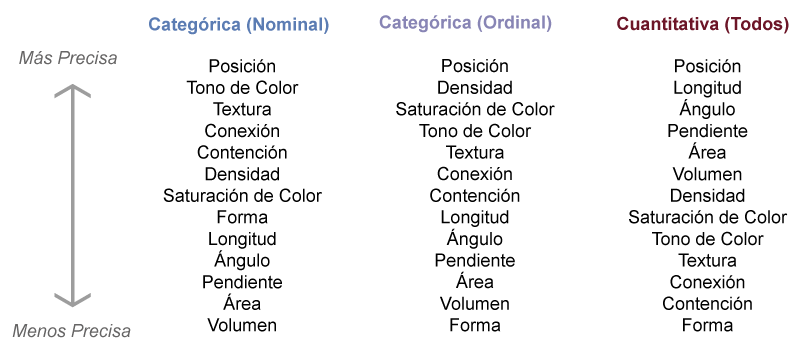
\includegraphics[width=0.95\textwidth]{fig17.png}
  \caption[Ranking de las tareas perceptivas]{Imagen recreada a partir de 'Ranking of Perceptual Tasks' de Jock MacKinlay \cite{Vie04}.}
  \label{fig:fig17}
\end{figure}

Estos estudios se enfocaron en el hecho de que nuestro sistema visual no es capaz de mediciones absolutas y por tanto, sólo se plantea una guía para entender cual variable va a ser mejor para entregar mediciones relativas con la mayor precisión.

\paragraph{Creación de una metáfora de diseño apropiada}
Una metáfora visual es una capa adicional de significado que se enfoca en transmitir un extra de conexión entre los datos, el diseño y el tema.

\paragraph{Selección de la solución final}
A partir de las opciones que procesamos en las tareas anteriores se puede identificar la especificación de la representación correcta de los datos para la visualización.

La clave es enfocarse en entregar los elementos funcionales apropiados mediante el uso de la representación de datos más adecuada para la visualización y dejar que la estética emerja como consecuencia de un buen diseño.

\subsubsection{Capa de presentación de los datos}
La presentación de los datos involucra las decisiones de diseño asociadas a todas aquellas características adicionales que podrían ser incluidas en la visualización. Estas son:

\begin{itemize}
  \item El uso del color
  \item La potencialidad de funciones interactivas
  \item Las anotaciones explicativas
  \item La arquitectura y disposición
\end{itemize}

Las decisiones que se hacen sobre estas capas deben enfocarse en proporcionar mayor significado, intuitividad y profundidad en la comprensión de los lectores o usuarios.

Uno de los conceptos claves para guiarse en la selección de opciones de diseño relacionadas con la presentación es hacer invisible aquello que es visible. Esto significa hacer que los elementos de presentación se sientan casi invisibles, tal que la ilustración de los datos preserve su dominio visual. En ese sentido, debe tenerse en mente dos cosas:

\begin{itemize}
  \item La inferencia visual se traduce en inferencia de datos.
  \item Los elementos visuales deben facilitar la discriminación de los datos.
\end{itemize}

\paragraph{El uso del color}

El mejor consejo para guiarse en el uso del color es asegurarse de que se usa de forma no intrusiva y que no conduzca erróneamente a interpretaciones cuando no debe. A continuación se muestran consideraciones para los siguientes tres casos de uso del color.

\subparagraph{Para representar datos}

Uno de los errores más comunes en el uso del color es el empleo de su propiedad del tono (hue) para representar datos cuantitativos. Esto es inapropiado ya que el ser humano no percibe un color como inherentemente más grande o pequeño que otro. Si se desea emplear el color para la representación de datos cuantitativos, es más efectiva la variación del brillo para un tono de color dado. A esto también se le conoce como esquema de color secuencial. Esta propiedad sí proporciona un sentido de los valores que son más altos y bajos, aunque es necesaria la incorporación de una leyenda que ayude a precisar valores absolutos. Más que obtener valores precisos, el sombreado de los patrones de mayor y menor valor es realmente el propósito principal del uso del color para representar datos cuantitativos.

Hay otros tipos de esquemas de color usados para situaciones que requieren la presentación de dos variables cuantitativas o para destacar los dos extremos de una sola variable. Éstos se conocen como esquemas divergentes, y por lo general presentan los extremos del espectro con colores oscuros y contrastantes.

Es importante tomar en cuenta que alrededor del 10\% de la población tiene una deficiencia en la percepción del color rojo y verde. Una alternativa efectiva en este caso es cambiar el verde por el azul.

Una de las funciones clave de una variable visual es facilitar la discriminación de los datos. El uso del tono de color para distinguir variables categóricas es particularmente efectivo. Sin embargo, es importante tomar en cuenta que el ojo es sólo capaz de distinguir hasta 12 clasificaciones de colores diferentes. El uso de una gama mayor puede dificultar la diferenciación de las distintas categorías.

\subparagraph{Traer los datos a un primer plano}

También se puede emplear el color para ayudar en la creación de un efecto de profundidad visual y una sensación de jerarquía en nuestros diseños. Básicamente se trata de traer los elementos más importantes a un primer plano y trasladar las menos importantes hacia el fondo. Un ejemplo de aplicación de esta técnica es el uso de un esquema de color monocromático que permita que otros tonos de color resalten al incorporarlos en aquellos aspectos que se quieren destacar.

En general, se recomienda no usar colores fuertes y altamente saturados al cubrir grandes áreas. En su lugar, es preferible usar estos colores para resaltar y llevar la atención a la capa de datos.

\subparagraph{Para adecuarse a requerimientos de diseño}

El factor final relacionado al color involucra la necesidad de incorporar la identidad visual de una organización mediante el uso de una paleta de color predefinida.

\paragraph{Creando interactividad}

Los avances de la tecnología en la última década han creado increíbles oportunidades para el desarrollo de poderosas visualizaciones interactivas. Los mejores diseños de interactividad se funden en el diseño de tal forma que el mecanismo de interacción es inseparable de la visualización de los datos.

El desarrollo de una visualización interactiva requiere de capacidades técnicas. Además, se debe tomar en cuenta la compatibilidad de la plataforma, la velocidad de carga de los datos y la capacidad del servidor.

La interactividad no siempre significa una experiencia de usuario mejorada. Por ello no se debe comprometer la esencia de la comunicación visual con el abandono del diseño estático por el simple hecho de crear interactividad. Un escenario apropiado para incorporar interactividad es cuando la complejidad y variedad de los datos son incompatibles con un diseño estático.

A continuación se muestra un resumen de la variedad de funciones y características que pueden considerarse en la construcción de una visualización interactiva.

\begin{description}
  \item[Manipulación de variables y parámetros:] es la habilidad de seleccionar, filtrar, excluir, o modificar ciertas variables para permitir al usuario interactuar con diferentes partes de los datos.
  \item[Ajuste de la vista:] tiene que ver con las capacidades de acercamiento del usuario hacia la visualización.
  \item[Animación:] es la inclusión de movimiento en la visualización. Esta técnica tiene gran potencial en datos basados en series temporales.
\end{description}

\paragraph{Anotaciones}

Las anotaciones ayudan a explicar y facilitan la experiencia visual e interpretativa. Es la capa de asistencia al usuario y de comprensión del usuario. Un objetivo clave del diseño de visualización de datos es facilitar la accesibilidad al tópico mediante un diseño intuitivo. El grado de accesibilidad se mejora con la inclusión de explicaciones útiles en todas las características de la visualización. No se debe asumir que el usuario podrá navegar con facilidad la visualización sin ninguna asistencia. Para ello se puede incluir con los siguientes elementos:

\begin{description}
  \item[Títulos:] pueden ayudar a atraer la atención de la audiencia y a articular el foco del tópico de la visualización.
  \item[Introducciones:] son importantes para explicar el trasfondo y contexto del proyecto.
  \item[Guías de usuario:] aunque la accesibilidad intuitiva es una meta fundamental, en algunos proyectos complejos es necesario hacer este tipo de anotaciones para dar mayor explicación al usuario.
  \item[Etiquetas:] revelan características extra y detalles sobre los datos.
  \item[Subtítulos y narrativa:] de manera complementaria con el título, estas anotaciones pueden ayudar a acelerar el proceso interpretativo y de compresión del usuario.
  \item[Anotaciones visuales:] son anotaciones que van más allá de ayudas textuales. Ejemplos de ellas son las cuadrículas, etiquetas de ejes, líneas de referencia y sombreado de fondo.
  \item[Leyendas:] explican los esquemas de color usados o los tamaños de las formas en términos de su representación categórica o cuantitativa.
  \item[Unidades:] deben incluirse detalles de las unidades de valor empleadas para evitar ambigüedades y malas interpretaciones.
  \item[Fuentes de los datos:] son referencias detalladas sobre dónde se obtuvieron los datos o cualquier otro elemento externo (como imágenes).
  \item[Atribuciones:] es el reconocimiento a personas que han contribuido directamente, influenciado la construcción del diseño o han servido de inspiración.
\end{description}

\paragraph{Disposición}

Es la capa final en la que se considera el acomodo del diseño en términos del formato, posicionamiento, y la organización de todos los elementos visibles. La intención con la disposición y arquitectura es proporcionar la experiencia más intuitiva posible. La meta es reducir la cantidad de trabajo que el ojo debe realizar para navegar en el diseño y descifrar la secuencia y jerarquía de la visualización. Deben considerarse con cuidado las elecciones en cuanto al tamaño, posicionamiento, agrupación y ordenamiento de todo lo que se muestre. Al igual que el resto de la capas de diseño, deben justificarse las decisiones de todas la propiedades visuales presentadas.

\section{La Práctica Gráfica}

En su libro "The Visual Display of Quantitive Information", Tufte \cite{Tuf83} postula los conceptos de excelencia gráfica e integridad gráfica, que son importantes como guías de evaluación de la calidad de una visualización de datos.

\subsection{Excelencia Gráfica}

La excelencia en los gráficos estadísticos consiste de ideas complejas comunicadas con claridad, precisión y eficiencia. Las visualizaciones deben:

\begin{itemize}
  \item Mostrar los datos.
  \item Inducir al usuario a pensar en la substancia en lugar de la metodología, diseño gráfico, tecnología o cualquier otra cosa.
  \item Evitar distorsionar los datos de cualquier manera.
  \item Presentar una gran cantidad de número en un espacio pequeño.
  \item Hacer coherentes un gran conjunto de datos
  \item Motivar al usuario a comparar diferentes trozos de datos.
  \item Mostrar los datos a distintos niveles de detalle, desde una visual amplia hasta la estructura fina.
  \item Servir a un propósito claro: descripción, exploración, tabulación o decoración.
  \item Estar integrado con la descripción estadística y verbal del conjunto de datos.
  \item Los gráficos "revelan" información sobre los datos.
\end{itemize}

\subsection{Integridad gráfica}

La integridad gráfica es el resultado de seis principios:

\begin{itemize}
  \item La representación de los números, deben ser proporcionales a las cantidades numéricas.
  \item Etiquetado minucioso, claro y detallado debe ser usado para atacar cualquier distorsión gráfica o ambigüedad.
  \item Mostrar variaciones en la data, no variaciones en diseño.
  \item El número de dimensiones mostradas no debe exceder el número de dimensiones de los datos.
  \item Los gráficos no deben citar datos fuera de contexto.
\end{itemize}
